% -*- coding: UTF-8 -*-
% vim: autoindent expandtab tabstop=4 sw=4 sts=4 filetype=tex
% vim: spelllang=de spell
% chktex-file 27 - disable warning about missing include files

\section{Darstellung von impliziten Oberflächen}
\label{sec:description_implicit_surfaces}

Nach~\citeauthor{hart_sphere_1994}, existieren verschiedene
Möglichkeiten zur Darstellung (zum Rendering) von impliziten
Oberflächen. So wandeln indirekte Methoden implizite Oberflächen in
Polygon-Modelle um, was die Nutzung bestehender Techniken und Hardware
zur Darstellung von polygonalen Modellen erlaubt. Die Umwandlung in
Polygon-Modelle ist jedoch nicht in jedem Falle gegeben. Sie kann zu
unzusammenhängenden Flächen oder zu einer Verminderung des
Detaillierungsgrades führen. Speicherbedarf und Zeitaufwand können zudem
sehr gross sein~\parencite[S.  528]{hart_sphere_1994}.

Eine andere Methode zur Darstellung von impliziten Oberflächen ist das
in~\autoref{subsec:ray_tracing} vorgestellte Ray Tracing Verfahren.

Ein (Licht-) Strahl wird dabei parametrisch als

\begin{gather}\label{eq:ray_param}
    r(t) = r_{0} + t \cdot r_{d}
\end{gather}

beschrieben. Der Strahl startet dabei bei Punkt $r_{0}$ in Richtung des
Einheitsvektors $r_{d}$, wobei $t$ die zurückgelegte Distanz des
Strahles ist.  Dabei ist $r(t)$ derjenige Punkt im Raum, welchen der
Strahl nach dem Zurücklegen der Distanz $t$ --- ausgehend von seinem
Ursprung $r_{0}$ --- erreicht~\parencite[S. 528]{hart_sphere_1994}.

Um nun die Schnittpunkte eines Strahles mit einer impliziten Oberfläche
zu finden, wird die Gleichung des Lichtstrahles $r$ (\ref{eq:ray_param})
in die Funktion einer impliziten Oberfläche $f$
(\ref{eq:surface_implicit}) eingesetzt. Wobei $r : \mathbb{R} \to
\mathbb{R}^{3}$ und $f : \mathbb{R}^{3} \to \mathbb{R}$. Dies ergibt die
zusammengesetzte Funktion $F = f \circ r$ wobei $F : \mathbb{R} \to
\mathbb{R}$~\parencite[S. 528]{hart_sphere_1994}.

Die Lösungen dieser Gleichung ergibt alle Distanzen $t$, welche ein
gegebener Strahl zurücklegt und welche die folgende Bedingung
erfüllen~\parencite[S. 528]{hart_sphere_1994}:

\begin{gather}\label{eq:ray_param_cond}
    F(t) = f \circ r = f(r(t)) = 0
\end{gather}

Für die Lösung der~\autoref{eq:ray_param_cond}, können numerische
Verfahren zur Suche von Nullstellen angewendet werden. Dabei sind die
Verfahren vom Typen der Funktion $F(t)$ abhängig. Bei polynomialen
Funktionen bis zum vierten Grad existieren analytische Lösungen.
Idealerweise genügt für das Finden der Nullstellen die Auswertung der
Funktion $F$ am Punkt $t$. Dabei können jedoch Nullstellen verloren
gehen~\parencite[S. 528]{hart_sphere_1994}.

Für eine beliebige Funktion $F(t)$ muss daher ein generisches, robustes
Verfahren zur Suche von Nullstellen verwendet werden. Eine solches
Verfahren benötigt jedoch zusätzliche Informationen und geht somit über
eine einfache Auswertung der Funktion hinaus. Die zusätzlichen
Informationen können zumeist aus der Ableitung der Funktion gewonnen
werden~\parencite[S. 528]{hart_sphere_1994}.

Ein häufiger Nachteil der erwähnten Verfahren Nullstellen-Suche ist,
dass sie mehrere Schnittpunkte eines Strahles mit einer impliziten
Oberfläche liefern. Zur Umgehung dieser Problematik, wird nur der
kleinste Wert von $t$ --- also der geringste Abstand ---
berücksichtigt~\parencite[S. 531]{hart_sphere_1994}.

Die Ray Marching und Sphere Tracing Algorithmen gehen hier sogar noch
einen Schritt weiter. Sie betrachten nur die kleinste positive Nullstelle
der~\autoref{eq:ray_param_cond}~\parencite[S. 531]{hart_sphere_1994}.

% -*- coding: UTF-8 -*-
% vim: autoindent expandtab tabstop=4 sw=4 sts=4 filetype=tex
% vim: spelllang=de spell
% chktex-file 27 - disable warning about missing include files

\subsection{Ray Marching}
\label{subsec:ray_marching}

~\citeauthor{perlin_hypertexture_1989} schlagen eine Abtastung des
Strahles mit fixen Abständen $\Delta \mu$ vor~\parencite[S.
259]{perlin_hypertexture_1989}:

\begin{gather}
    x = x_{\mu_{0}} + k \cdot \Delta x_{\mu}
\end{gather}

Dabei ist $k = 0,1,2,\dots$ und $\mu_{0} + k \Delta \mu \leq \mu_{1}$.

Auf die parametrische Darstellung eines (Licht-) Strahles,
~\autoref{eq:ray_param_cond}, angewendet, ergibt dies folgende Gleichung:

\begin{gather}
    r(k) = r_{0} + \Delta t \cdot k \cdot r_{d}
\end{gather}

Dabei stellt $\Delta t$ die Grösse der Abstände und $k = 0,1,2,\dots$ die Nummer der
Schritte dar. Wie~\citeauthor{hart_ray_1989} schreiben, bildet das Abtasten des
(Licht-) Strahles mit fixen Abständen die Basis für gewisse Verfahren des
volumetrischen Renderings~\parencite[S. 291]{hart_ray_1989}.

Ein möglicher Algorithmus, wie solch ein Verfahren umgesetzt werden kann,
findet sich in~\autoref{fig:ray_marching}.

\begin{lstlisting}[language=Python,caption={Eine abstrakte Umsetzung des Ray
        Marchings\protect\footnotemark.},label={fig:ray_marching},captionpos=b,emph={ray_march}]
def ray_march():
    step         = 0
    intersection = 0
    max_steps    = 10

    while step < max_steps:
        intersection = test_intersection(k)

        if intersection <= 0:
            # An intersection has happened
            #   intersection <  0: ray is inside surface
            #   intersection == 0: ray is excatly on surface
            return ray_travel_distance(step)

        step = step + 1

    # When we reach this step, after max_steps, no intersection
    # has happened, so distance is 0
    return 0
\end{lstlisting}
\footnotetext{Algorithmus in Pseudocode
    gemäss~\cite{perlin_hypertexture_1989}[S. 259, Abschnitt 3.1]}

Dabei ist zu beachten, dass der Abstand der Abtastung eines Strahles
$\Delta{t}$ so gering als möglich sein sollte um eine Menge von Punkten bzw.\ ein
Objekt $A$ --- definiert durch implizite Oberflächen --- möglichst gut
abschätzen zu können. Ist der Abstand zu gross gewählt, so findet ggf.
eine Abtastung weit im Inneren des Objektes statt. Damit geht Präzision
verloren. Es ist weiter möglich, dass der erste eigentliche Punkt gar nicht
abgetastet wird und erst der zweite abgetastete Punkt das Objekt ``erkennt''.

\begin{figure}[H]
    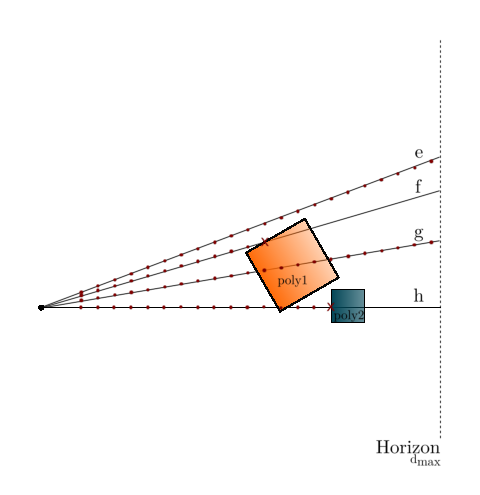
\includegraphics[width=0.8\textwidth]{img/ray_marching_problems.pdf}
    \caption{Illustration des Ray Marching Verfahrens und dessen
        Problematiken.\protect\footnotemark}\label{fig:ray_marching_problems}
\end{figure}
\footnotetext{Eigene Darstellung mittels Inkscape.}

\autoref{fig:ray_marching_problems} veranschaulicht diese
Problematiken. Zu sehen sind vier Primärstrahlen, \textit{e},
\textit{f}, \textit{g} und \textit{h},  sowie zwei Objekte,
\textit{poly1} und \textit{poly2}.

Bei den Strahlen \textit{e} und \textit{f} handelt es sich um
``normale'' Fälle: Der Strahl \textit{e} verfehlt beide Objekte;
das Ray Marching wird also nach Erreichen der maximalen Distanz
\textit{d\textsubscript{max}} abgebrochen.\\
Der Strahl \textit{f} trifft das Objekt \textit{poly1} nach 12
Schritten.

Die Strahlen \textit{g} und \textit{h} sind Spezialfälle: Der Strahl
\textit{g} geht durch das Objekt \textit{poly1}, erfasst dieses wegen
des gewählten fixen Abstandes der Abtastungspunkte ($\Delta{t}$) nicht.

Der Strahl \textit{h} liefert das Objekt \textit{poly2}, obwohl er
eigentlich das Objekt \textit{poly1} liefern müsste. Das getroffene
Objekt \textit{poly2} dürfte so gar nicht zu sehen sein. Dieser Fehler
tritt wiederum aufgrund des gewählten fixen Abstandes der Abtastpunkte
($\Delta{t}$) auf.

\citeauthor{hart_sphere_1994} weist darauf hin, dass Ray Marching durch
den möglichst geringen Abstand zwischen den Abtastungen entsprechend
langsam und paralleles Abtasten praktisch unumgänglich ist~\parencite[S.
528]{hart_sphere_1994}. In der von~\citeauthor{hart_sphere_1994} vorgestellten
Technik des Sphere Tracings ist der Abstand zwischen den Abtastungen
nicht konstant sondern variiert in Abhängigkeit der
Geometrie~\parencite[S. 538 bis 540]{hart_sphere_1994}.

% -*- coding: UTF-8 -*-
% vim: autoindent expandtab tabstop=4 sw=4 sts=4 filetype=tex
% vim: spelllang=de spell
% chktex-file 27 - disable warning about missing include files

\subsection{Sphere Tracing}
\label{subsec:sphere_tracing}

Das von~\citeauthor{hart_sphere_1994} vorgeschlagene Sphere Tracing
Verfahren ist ein~\hyperref[subsec:ray_tracing]{Ray Tracing} Verfahren
für~\hyperref[subsec:implicit_surfaces]{implizite Oberflächen}. Es ist
ebenfalls ein~\hyperref[subsec:ray_marching]{Ray Marching} Verfahren.
Jedoch wird die Distanz der Abtastungsschritte eines (Licht-) Strahles
aufgrund einer~\hyperref[ssubsec:distance_functions]{Distanzfunktion}
bestimmt.
Das Verfahren wurde erstmalig~\citeyear{hart_ray_1989}
in~\citetitle{hart_ray_1989} von~\citeauthor{hart_ray_1989}
vorgestellt~\parencite{hart_ray_1989}.

Ein möglicher Algorithmus, wie Sphere Tracing umgesetzt werden kann,
findet sich in~\autoref{alg:sphere_tracing}.

Bei Sphere Tracing werden die Schnittpunkte eines (Licht-) Strahles
durch eine Folge von negativen Hüllkörpern (``unbounding volumes'') ---
bzw.\ in diesem Fall Kugeln (``unbounding spheres'') --- beschrieben.
Davon kommt die Bezeichnung Sphere Tracing~\parencite[S.
530]{hart_sphere_1994}.

``Unbounding volumes'' (zu Deutsch etwa ``negativer Hüllkörper'') wird
von den Autoren~\citeauthor{hart_ray_1989} benutzt, um das Sphere
Tracing Verfahren zu beschreiben und darzustellen. Der Term steht im
Gegensatz zu dem gängigen Konzept des Hüllkörpers (``bounding volume'').
Bei einem Hüllkörper wird ein Körper umschlossen. Der ``negative
Hüllkörper'' umschliesst ein Stück des Raumes ohne dabei ein Objekt zu
umschliessen (dass heisst ohne ein gesuchtes Objekt zu
``berühren'')~\parencite[S. 291]{hart_ray_1989}. Die ``negativen
Hüllkörper'' sind in~\autoref{fig:sphere_tracing_1} als Kreisflächen
dargestellt.

Für die Berechnung eines negativen Hüllkörpers sucht man
den Abstand eines Objektes von einem Ausgangspunkt.
Ist die kürzeste Distanz zwischen Ausgangspunkt und
Objekt bekannt, kann diese als Radius einer Kugel angenommen werden. 

Objekte sind bei dem genannten Verfahren durch Distanzfunktionen
definiert. So ist z.B. eine Kugel als Punkt im Raum minus deren Radius
definiert (siehe~\autoref{eq:surface_immplicit_geometric}). Der
Betrachter kann dabei auch als Punkt im Raum angenommen werden. Somit
sind alle Distanzen bekannt (siehe auch
Distanzfelder,~\autoref{ssubsec:distance_fields}).

Eine Kugel dient als negativer Hüllkörper (``unbounding Volume''). Sie
ist aber \textit{nicht} Teil des Objektes und schneidet dieses
auch nicht (ist also nicht $\overset{\circ}{\bm{A}}$).\\
Nur der äusserste Punkt des Abstandes  liegt genau
auf der Oberfläche des Objektes ($\partial \bm{A}$). Der Radius einer
solchen Kugel wird durch Evaluation der Distanzfunktion eines
abzutastenden Punktes im Raum bestimmt.

\citeauthor{hart_ray_1989} beschreiben in ihrer
Arbeit~\citetitle{hart_ray_1989} die Darstellung von Fraktalen im
dreidimensionalen Raum. Es wird von einer Abschätzung der Distanz
gesprochen, da diese für Fraktale nicht effizient berechnet werden
kann~\parencite[S.  291]{hart_ray_1989}.\\
Bei ``regulären'' Objekten, wie z.B. einer Kugel, kann der zur
Oberfläche am nächsten gelegene Punkt von einem beliebigen Punkt
derselben Domäne exakt berechnet werden~\parencite[S.
530]{hart_sphere_1994}. Dies ist durch die
implizite~\autoref{eq:surface_implicit_sphere} gegeben.

Gemäss~\cite[S. 291 - 292]{hart_ray_1989} geschieht die Verfolgung der
Strahlen bei Sphere Tracing wie folgt: Ein Strahl wird vom Betrachter
(Auge bzw.  Lochkamera) durch die Bildebene zu einem Objekt geschossen.
Dabei wird bei dem initialen Ausgangspunkt der Radius eines negativen
Hüllkörpers in Form einer ersten Kugel berechnet, so wie oben beschrieben.
Dies ist die Distanz, welche der Strahl in einem ersten
Schritt effektiv zurücklegen wird. Von diesem Schnittpunkt aus wird
erneut der Radius einer Kugel berechnet usw.

Dies geschieht so lange, bis der Strahl schliesslich von einem
Schnittpunkt des negativen Hüllkörpers aus auf die Oberfläche eines
Objektes trifft.\\
Ein weiteres Kriterium für den Abbruch ist eine vordefinierte maximale
Distanz des Strahles ($d_{\text{max}}$). Ist diese erreicht und der
Strahl verfehlt die Oberfläche des Objektes, wird abgebrochen. Somit ist
auch ersichtlich, dass Sphere Tracing nicht die genannten Problematiken
von Ray Marching aufweist (siehe~\autoref{subsec:ray_marching}).

Die folgenden Abbildungen~\ref{fig:sphere_tracing_1}
und~\ref{fig:sphere_tracing_2} veranschaulichen das Sphere Tracing
Verfahren.

\begin{figure}[H]
    \centering
    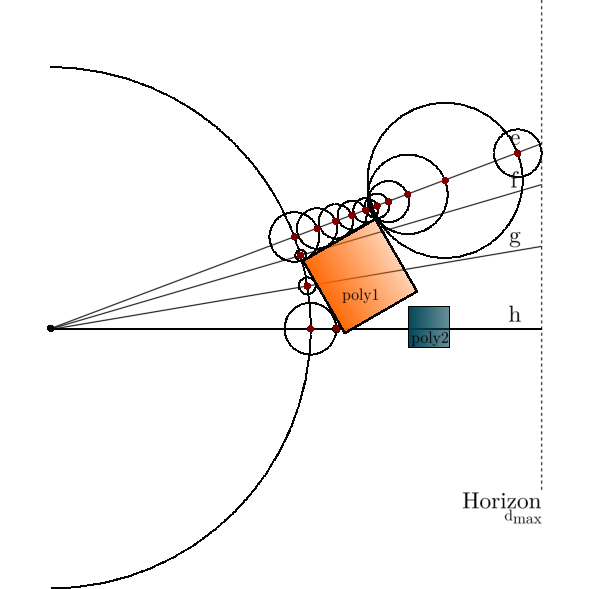
\includegraphics{img/sphere_tracing_principle.pdf}
    \caption{Illustration des Sphere Tracing
        Verfahrens.\protect\footnotemark}\label{fig:sphere_tracing_1}
\end{figure}
\footnotetext{Eigene Darstellung mittels Inkscape.}

\begin{figure}[H]
    \centering
    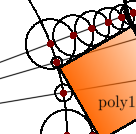
\includegraphics[width=0.5\textwidth]{img/sphere_tracing_principle_near.pdf}
    \caption{Illustration des Sphere Tracing Verfahrens,
        Nahaufnahme.\protect\footnotemark}\label{fig:sphere_tracing_2}
\end{figure}
\footnotetext{Eigene Darstellung mittels Inkscape.}

Ausgehend von der parametrischen Beschreibung eines (Licht-) Strahles
(\autoref{eq:ray_param}), beschreiben~\citeauthor{hart_ray_1989} die
Richtung $r_{d}$ eines Strahles als Einheitsvektor~\parencite[S.
291]{hart_ray_1989}:

\begin{gather}
    r_{d} = \frac{p_{x, y} - r_{0}}{|p_{x, y} - r_{0}|}
\end{gather}

Dabei ist $r_{0}$ der Ursprung eines Strahles und $p_{x, y}$ ein Punkt
der Bildebene.

Um nun den Schnittpunkt eines Strahles $r_{d}$ mit der Oberfläche eines
Objektes zu finden, muss~\autoref{eq:ray_param_cond}, $F(t) = f \circ
r = 0$, gelöst werden. Dabei ist --- wie oben definiert --- die Funktion
$f(x)$ nun eine Distanzfunktion, wie zum Beispiel die geometrische
Distanzfunktion zur Beschreibung einer Kugel
(\autoref{eq:surface_immplicit_geometric}).

Evaluiert man nun die Gleichung $F(t)$ unter Anwendung der eben beschriebenen
Verfolgung der Strahlen, findet man so die erste positive Nullstelle der Gleichung
$F(t)$. Diese Nullstelle ist die Grenze der Folge von negativen Hüllkörpern
(``unbounding spheres''), welche durch die rekursive Gleichung:

\begin{gather}
    t_{i+1} = t_{i} + F(t_{i})
\end{gather}

definiert ist. Der Ursprungspunkt ist dabei als $t_{0}$ definiert. Diese Folge
konvergiert genau dann --- und nur dann --- wenn der Strahl auf die implizite
Oberfläche eines Objektes trifft. Diese Folge bildet den Kern des Algorithmus
zur Darstellung von geometrisch definierten, impliziten Oberflächen.

\begin{minipage}{\linewidth}
\begin{lstlisting}[language=Python,caption={Eine abstrakte Umsetzung des Sphere
        Tracings\protect\footnotemark.},label={alg:sphere_tracing},captionpos=b,emph={sphere_trace}]
def sphere_trace():
    ray_distance          = 0
    estimated_distance    = 0
    max_distance          = 9001
    convergence_precision = 0.000001

    while ray_distance < max_distance:
        # sd_sphere is a signed distance function defining the implicit surface
        # cast_ray defines the ray equation given the current travelled /
        # marched distance of the ray
        estimated_distance = sd_sphere(cast_ray(ray_distance))

        if estimated_distance < convergence_precision:
            # the estimated distance is already smaller than the desired
            # precision of the convergence, so return the distance the ray has
            # travelled as we have an intersection
            return ray_distance
        # end if

        ray_distance = ray_distance + estimated_distance
    # done while

    # When we reach this point, there was no intersection between the ray and a
    # implicit surface, so simply return 0
    return 0
# end def sphere_trace
\end{lstlisting}
\footnotetext{Algorithmus in Pseudocode gemäss~\cite{hart_sphere_1994}[S. 531,
    Fig. 1]}
\end{minipage}

% -*- coding: UTF-8 -*-
% vim: autoindent expandtab tabstop=4 sw=4 sts=4 filetype=tex
% vim: spelllang=de spell
% chktex-file 27 - disable warning about missing include files

\subsection{Operationen für implizite Oberflächen}
\label{subsec:implicit_surfaces_ops}

Um mit impliziten Oberflächen nicht nur einfache Objekte wie
beispielsweise eine Kugel darstellen zu können muss man diese auch
transformieren können.

Wie~\citeauthor{hart_sphere_1994} beschreibt, werden implizite
Oberflächen durch die Invertierung des Raumes, in welchem sich eine
Oberfläche befindet, transformiert~\parencite[S. 543]{hart_sphere_1994}.
Der Raum, in dem sich eine implizite Oberfläche befindet, ist die Domäne
der impliziten Funktion der Oberfläche.

Sei $T(\bm{x})$ eine Transformation und $f(\bm{x})$ eine Distanzfunktion,
welche eine implizite Oberfläche definiert. Somit ist die transformierte
implizite Oberfläche~\parencite[S. 534]{hart_sphere_1994}:

\begin{gather}
    f(T^{-1}(\bm{x})) = 0
\end{gather}

Bei Transformationen handelt es sich um von dem Vorzeichen abhängige
Distanzfunktionen (\textit{signed distance functions}).

Es werden folgende Arten von Transformationen
unterschieden~\parencite[S. 14]{hart_ray_1993}:
\begin{itemize}
    \item{Distanz-Operationen}\\
        Zum Beispiel Vereinigung, Subtraktion oder Intersektion.
    \item{Domänen-Operationen}\\
        Zum Beispiel Wiederholung, Rotation, Translation und Skalierung.
    \item{Distanz-Deformationen}\\
        Zum Beispiel Versatz (displacement) und Vermengung/Vermischung.
        (\textit{blend})
    \item{Domänen-Deformationen}\\
        Zum Beispiel ``Verwindung'' (\textit{twist}) und Biegung
        (\textit{bend}).
\end{itemize}

\subsubsection{Isometrien}
\label{ssubsec:implicit_surfaces_ops_isometries}

Nicht alle Transformationen erhalten dabei die Distanz, welche die
Distanzfunktion der transformieren Oberfläche zurückgeben würde. In
solch einem Falle ist die zurückgegebene Distanz nicht die Distanz eines
beliebigen Punktes im Raum zu dem ihm nächsten Punkt einer impliziten
Oberfläche.

Transformationen, welche die Distanz hingegen erhalten,
bezeichnet~\citeauthor{hart_sphere_1994}
als~\textit{Isometrien}~\parencite[S. 534]{hart_sphere_1994}. Dazu
zählen Rotationen, Translationen aber auch Reflexionen.

Ist $\bm{I}$ eine Isometrie, dann benötigt die zurückgegebene Distanz der
Distanzfunktion $f(\bm{x})$ \textit{keine Anpassung}.

\begin{gather}
    d(\bm{x}, \bm{I} \circ f^{-1}(0)) = d(\bm{I}^{-1}(\bm{x}), f^{-1}(0))
\end{gather}

Wobei $\bm{I}$ eine Isometrie und $f^{-1}(0)$ eine implizite Oberfläche ist.

\subsubsection{Uniforme Skalierung}
\label{ssubsec:implicit_surfaces_ops_scaling}

Eine Skalierung bewahrt keine Distanzen. Somit muss die zurückgegebene
Distanz einer Distanzfunktion entsprechend angepasst werden.

\citeauthor{hart_sphere_1994} gibt die uniforme Skalierung als
Transformation $\bm{S(x)}$  der Form~\parencite[S. 534]{hart_sphere_1994}:

\begin{gather}
    \bm{S(x)} = s \cdot \bm{x}
\end{gather}

an, wobei $s$ der Skalierungsfaktor ist. Die Invertierung der Skalierung
ist gegeben als~\parencite[S. 534]{hart_sphere_1994}:

\begin{gather}
    \bm{S^{-1}(x)} = {1 \over s} \cdot \bm{x}
\end{gather}

Somit ist die Distanz zu der skalierten impliziten
Oberfläche~\parencite[S. 534]{hart_sphere_1994}:

\begin{gather}
    d(\bm{x}, \bm{S}(f^{-1}(0))) = s \cdot d(\bm{S}^{-1}(\bm{x}), f^{-1}(0))
\end{gather}

Dabei wird die von der Distanzfunktion der skalierten impliziten Oberfläche
zurückgegebene Distanz mit dem Skalierungsfaktor $s$ multipliziert, was die
eigentliche Information der Distanz erhält und die Skalierung somit isometrisch
macht.

\subsubsection{``Verwindung'' (\textit{Twist})}
\label{ssubsec:implicit_surfaces_ops_twist}

Gemäss~\citeauthor{hart_sphere_1994} werden bei der ``Verwindung''
(\textit{Twist}) einer impliziten Oberfläche zwei Achsen (z.B. $x$ und
$y$) anhand einer linearen Funktion $a(\cdot)$ in Abhängigkeit der
dritten Achse (z.B. $z$) rotiert~\parencite[S. 543]{hart_sphere_1994}:

\begin{gather}
    twist(\bm{x}) = \begin{pmatrix} 
        x \cdot \cos{a(z)} - y \cdot \sin{a(z)},\\
        x \cdot \sin{a(z)} + y \cdot \cos{a(z)},\\
        z
    \end{pmatrix}
\end{gather}

\subsubsection{Vereinigung}
\label{ssubsec:implicit_surfaces_ops_union}

Die Vereinigung zweier impliziter Oberflächen $A$ und $B$ wird
von~\citeauthor{hart_sphere_1994} als minimale Distanz der jeweiligen,
vom Vorzeichen abhängigen Distanzfunktion $f_{A}$ respektive $f_{B}$
definiert~\parencite[S. 531 bis 532]{hart_sphere_1994}:

\begin{gather}
    d(\bm{x}, A \cup B) = \min(f_{A}(\bm{x}), f_{B}(\bm{x}))
\end{gather}

Dabei $\bm{x}$ den abzutastenden Punkt im Raum darstellt.

\todo[inline]{Redigieren}
Wie~\citeauthor{hart_sphere_1994} schreibt, ist die Distanz zu einer
Menge von Objekten die kürzeste der Distanzen zu jedem der
zusammengesetzten Objekte.
\todo[inline]{/Redigieren}

Somit erlaubt die Vereinigung die Kombination von mehreren impliziten
Oberflächen, ohne dass diese miteinander in Kontakt stehen. So kann
beispielsweise eine komplexe Szene modelliert werden.

\todo[inline]{Bild von Vereinigung}

\subsubsection{Subtraktion}
\label{ssubsec:implicit_surfaces_ops_subtraction}

Für die Subtraktion wird die Distanz zum Komplement eines Objektes
$\bm{A}$ verwendet. Dabei wird die Eigenschaft der Abhängigkeit vom 
Vorzeichen der entsprechenden Distanzfunktionen genutzt~\parencite[S.
532]{hart_sphere_1994}:

\begin{gather}
    d(\bm{x}, \mathbb{R}^{3} \setminus A) = -f_{A}(\bm{x})
\end{gather}

Somit kann die Subtraktion zweier impliziter Oberflächen $A$ und $B$
gemäss~\citeauthor{hart_sphere_1994} als Intersektion eines Objektes $A$ mit der
Subtraktion des Raumes bzw.\ der Domäne mit einem Objekt $B$ angesehen werden,
daher folgt~\parencite[S. 532]{hart_sphere_1994}:

\begin{align}
    d(\bm{x}, A - B) &= A \cap (\mathbb{R}^{3} \setminus B) \\
                     &\geq \max(f_{A}(\bm{x}), -f_{B}(\bm{x}))
\end{align}

Dabei stellt $\bm{x}$ den abzutastenden Punkt im Raum dar.

\todo[inline]{Bild von Subtraktion}

\subsubsection{Intersektion}
\label{ssubsec:implicit_surfaces_ops_intersection}

Die Intersektion zweier impliziter Oberflächen $A$ und $B$ wird
von~\cite{hart_sphere_1994} als minimale Distanz der jeweiligen
vorzeichenabhängigen  Distanzfunktion $f_{A}$ respektive $f_{B}$
definiert~\parencite[S. 532]{hart_sphere_1994}:

\begin{gather}
    d(\bm{x}, A \cap B) \geq \max(f_{A}(\bm{x}), f_{B}(\bm{x}))
\end{gather}

wobei $\bm{x}$ den abzutastenden Punkt im Raum darstellt.

\subsection{Primitive}
\label{subsec:implicit_surfaces_primitives}

\citeauthor{hart_sphere_1994} führt in seiner Arbeit einige
(geometrische) Primitive auf, welche nachfolgend erläutert
werden~\parencite[S. 540ff]{hart_sphere_1994}.

\subsubsection{Ebene}
\label{ssubsec:implicit_surfaces_primitives_plane}

Die von dem Vorzeichen abhängige Distanz zu einer Ebene $P$ mit einer
Einheitsnormalen $\bm{n}$, welche sich mit dem Punkt $\bm{n} \cdot r$
schneidet ist wie folgt definiert:

\begin{gather}
    d(\bm{x}, P) = \bm{x} \cdot \bm{n} - r
\end{gather}

wobei $r$ die relative Positionierung der Ebene --- unter Einbezug der
Normalen der Ebene im Verhältnis zur Einheitsnormalen $\bm{n}$ --- im
Raum darstellt.

\subsubsection{Kugel}
\label{ssubsec:implicit_surfaces_primitives_sphere}

Eine Kugel ist als eine Menge von Punkten (Locus) in fixem Abstand eines
gegebenen Punktes. Die von dem Vorzeichen abhängige Distanz zu einer
Kugel $S$, ausgehend vom Ursprung, ist wie folgt:

\begin{gather}
    d(\bm{x}, S) = \|\bm{x}\| - r
\end{gather}

wobei $r$ den Radius der Kugel darstellt.

\subsubsection{Zylinder}
\label{ssubsec:implicit_surfaces_primitives_cylinder}

Die Distanz zu einem um die Z-Achse zentrierten Zylinder mit
Einheitsradius wird durch Projektion auf die XY-Ebene und Messung der
Distanz zum Einheitskreis berechnet:

\begin{gather}
    d(\bm{x}, Cyl) = \|(x, y)\| - r
\end{gather}

wobei $r$ den Radius des Zylinders und $\bm{x}$ den Punkt $(x,y,z)$ im
Raum darstellt.

\subsubsection{Kegel}
\label{ssubsec:implicit_surfaces_primitives_cone}

Die Distanz zu einem Kegel, welcher am Ursprung zentriert und entlang
der Z-Achse orientiert ist, wird wie folgt berechnet:

\begin{gather}
    d(\bm{x}, Cone) = \|(x, y)\| \cdot \cos(\phi) - |z| \cdot \sin(\phi)
\end{gather}

wobei $\phi$ den Winkel zur Z-Achse darstellt.

\subsubsection{Torus}
\label{ssubsec:implicit_surfaces_primitives_torus}

Beim Torus handelt es sich um das Produkt zweier Kreise, sowie den Abstand der Kreise:

\begin{gather}
    d(\bm{x}, T) = \|(\|(x, y)\| - R, z)\| - r
\end{gather}

wobei $R$ den äusseren Radius und $r$ den innerern Radius des Torus darstellt.
Der Torus ist am Ursprung zentriert und dreht sich um die Z-Achse.

